\FloatBarrier
\subsection{Daten und Analyse Kondensator}


\begin{figure}
	\centering
	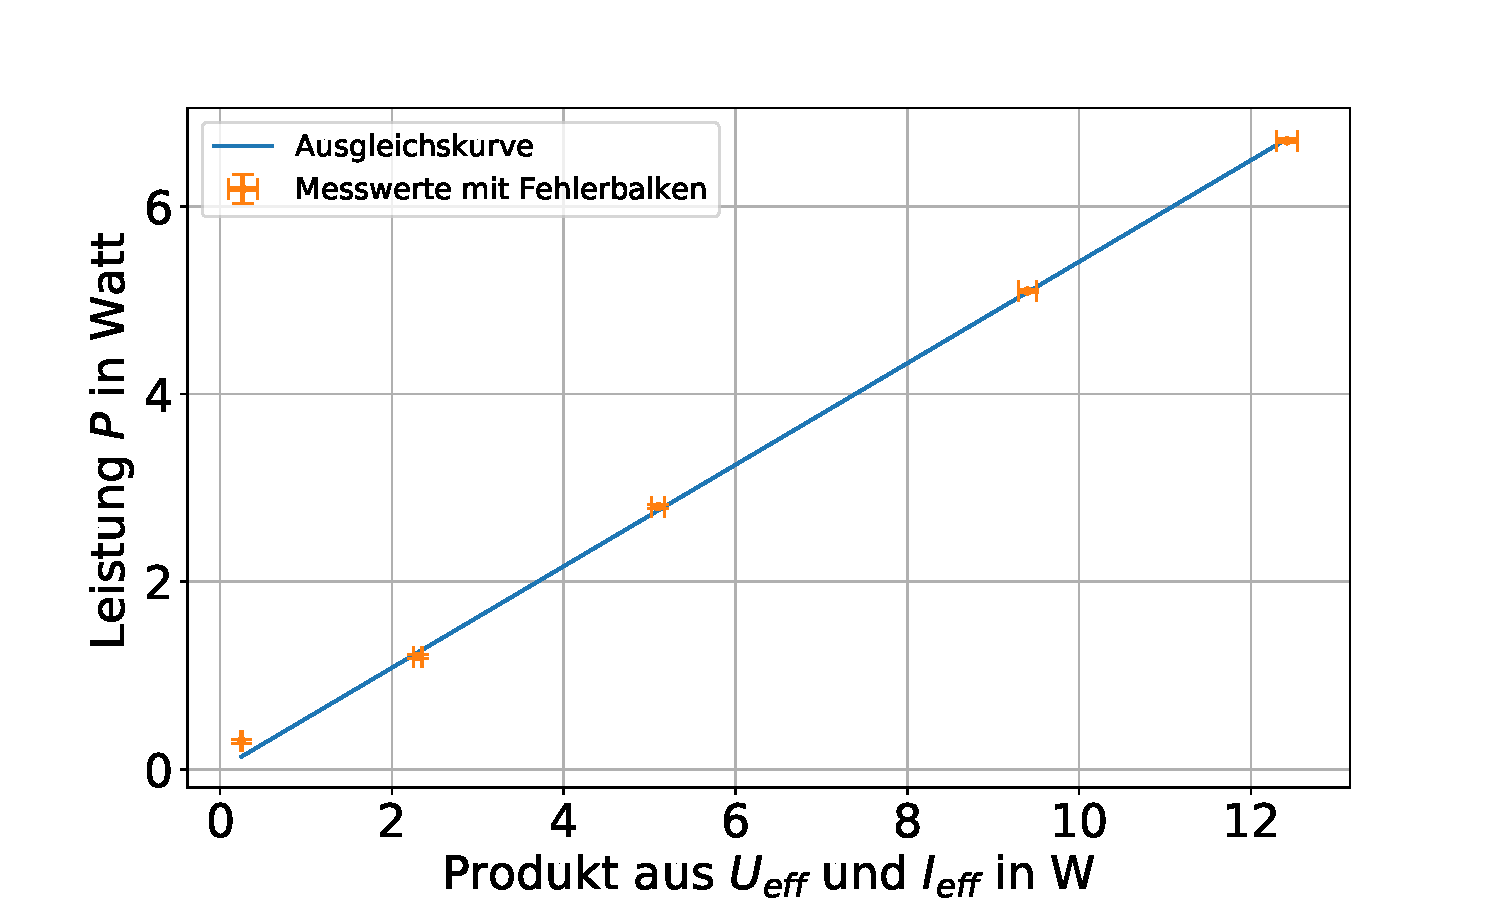
\includegraphics[width=0.9\textwidth]{res/PgegenUIK.pdf}
	\caption{Produkt aus Spannung $U$ und Strom $I$ gegen die Leistung $P$.}
	\label{fig:PgegenUIK}
\end{figure}


\begin{figure}
	\centering
	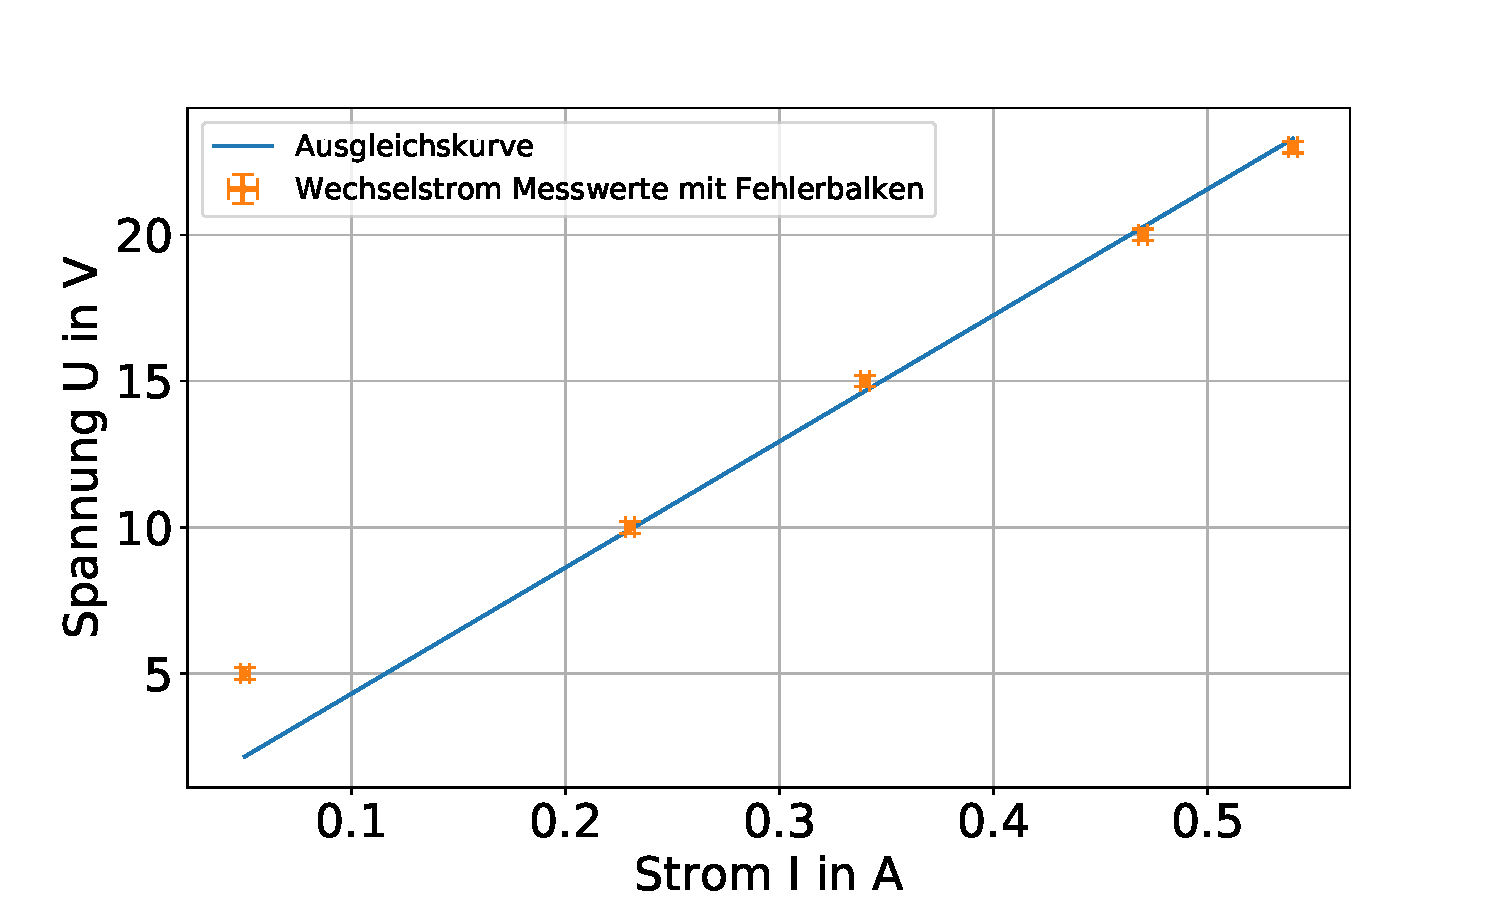
\includegraphics[width=0.9\textwidth]{res/UgegenIK.pdf}
	\caption{Spannung $U$ gegen den Strom $I$}
	\label{fig:UgegenIK}
\end{figure}


In diesem Teil des Protokolls wird die Kapazität~$C$, der Scheinwiderstand~$|Z|$ und der Phasenwinkel~$|\phi| $ der schon in Kapitel \ref{kap:MethodenS} beschriebenen Schaltung c). 
Dazu wurde zum einem der Innenwiderstand $R_i$ und die Induktivität $L$ der Spule aus der Auswertung aus Kapitel \ref{kap:Spule}.
Im Folgenden wird mit Hilfe der Abbildungen \ref{fig:PgegenUIK} und \ref{fig:UgegenIK}
und den Gleichungen:

\begin{align}
C=\frac{1}{\omega (\omega L+\sqrt{Z^2-R^2})}\\	
|\phi| = \arccos\left(\frac{\bar{P}}{U_{eff.}I_{eff.}}\right)\\
	|Z|=\frac{U_{eff.}}{I_{eff.}}
\end{align}
die Kapazität $C$ des Kondensators, der Betrag des Scheinwiderstandes und der Betrag der Phase berechnet. Das Ergebnis für die Kapazität wird mit den Herstellerangaben verglichen.Die angegebene Kapazität beträgt \SI{60+-3}{\mu F}.
Dieser Wert liegt in der $1\sigma$-Umgebung des errechneten Wertes: \SI{57+-4}{\mu F} und bestätigt die Angabe des Herstellers.
%Die für diese Rechnung nötigen Ergebnisse für die Phase und den Scheinwiderstand lauten:
%Die für die Berechnung der Kapazität benötigten
Der für die obige Rechnung benötigte Scheinwiederstand beträgt hier $	|Z| =\SI{43+-3}{\ohm}$. Des weiteren wird der Betrag der Phase~$|\phi| =\SI{0.9989+-0.0006}{rad}$ berechnet.\\
%\begin{align}
%	|\phi| &=\SI{0.9989+-0.0006}{rad}\\
%	|Z| &=\SI{43+-3}{\ohm}.
%\end{align}
Um die Unsicherheiten der Werte zu erhalten wurde für den Herstellerwert die von diesem angegebene Unsicherheit von $10\%$ nach Gleichung
\ref{eq:sur} abgeschätzt und die anderen Unsicherheitsrechnungen sind im Anhang~\ref{kap:Unsich} zu finden.
